%=== CHAPTER TWO (2) ===
%=== Literature Review ===

\chapter{Literature Review}

\section{Visual SLAM}

\subsection{Introduction}
Simultaneous Localizaiton and Mapping (SLAM) is a technique to obtain 3D structure of an unknown environment and sensor motion in the environment. After years of development, SLAM-based application have become widely broadened such as computer vision based 3D modeling, augmented reality(AR)-based visualization and self-driving cars. 

In early SLAM algorithms, there exit many different modalities of sensors integrated in SLAM systems, such as rotary encoders, light detection and ranging radar (LiDAR), inertial sensors, GPS and cameras. In recent years, SLAM using cameras only,  specifically referred to as visual SLAM (vSLAM), has been actively discussed because the sensor configuration is simple, low-cost, and contains abundant information. But meanwhile this technique also brings more difficulties than others using integrated sensors\cite{taketomi2017visual}. 

vSLAM algorithms have proposed widely in the field of computer vision, robotics and AR. The low requirement on the modalities of sensors, requiring cameras only, is the major advantage of vSLAM technique, so that it is very suitable for low-cost unmanned vehicles, robots with limited load capacity and power supply like drones, or mobile devices such as camera-mounted tablets or smart phones.

However, the difficulties brought by vSLAM can not be ignored. Instead of obtaining depth and location information directly from LiDAR, GPS or depth camera in integrated SLAM systems, vSLAM technique needs to compute all these information from color or gray images, which reduces stability and accuracy for several estimation steps involved in this process. Also obviously the computational cost are significantly higher. Therefore, the problem of how to improve the performance and reduce computational cost of vSLAM has always been widely concerned.


\subsection{Framework}

The framework of visual SLAM is mainly composed of three modules as follows:
\begin{enumerate}[1.]
	\item Sensor Data Collection
	\item Visual Odometry
	\item Global Map Optimization
	\item Loop Detection
	\item Mapping
\end{enumerate}
 This framework is illustrated in Figure \ref{fig:vslamframe}.

\begin{figure}[!ht]
  \centering
 % \hspace*{-135pt}
  \begin{tikzpicture}[node distance = 2cm, auto]
    % nodes
    \node [block] (init) { Sensor Data Collection};
    \node [block, below of = init] (contact) { Visual Odometry};
    \node [block, below of = contact] (consent) { Global Map Optimization};
    \node [block, below of = consent] (screening) { Mapping};
  \node [block, right of =contact, node distance =5cm](lc){ Loop Detection};
    % edges
    \path [line] (init) -- (contact);
    \path [line] (contact) -- (consent);
    \path [line] (consent) -- (screening);
    \path[line](init)--(lc);
   \path[line](lc)--(consent);
      \end{tikzpicture}
      \caption{Classic structure of Visual SLAM}
      \label{fig:vslamframe}
\end{figure}

Sensor data collection module in visual SLAM systems, is responsible to read and preprocess the image information collected from cameras.

In the module of visual odometry, the reconstrcuted map is tracked in the image to estimate the camera pose of the image with respect to the map. In order to do this, feature tracking or feature matching is executed to obtain 2D-3D correspondences between the image and the map. Then, the camera pose is computed by solving the Perspective-n-point (PnP) problem from the correspondences \cite{klette1998three,nister2007minimal}.

The other module is loop detection, or loop closing, which is a technique to acquire the reference information. In this module, loop closure is detected by matching a current image with previously acquired images. if a closed loop is detected, it means one of the previously observed place is revisited. In this case, the accumulative error can be estimated. The closed loops and the estimated accumulative error will be sent to the next module of global map optimization.

The next module is global map optimization. The reconstructed map includes accumulative estimation error according to the movement distance of the camera. To suppress the accumulative error, the global map optimization is usually performed. In this module, the map is refined according to the consistency of the entire map. When a place is revisited and a closed loop is detected, reference information that represents the accumulative error can be computed. Then global map optimizer can suppress the accumulative error using loop closure from the reference information as a constraint.

Mapping is the last module. In this module, the map is constructed and expanded by computing the 3D structure of the environment according to the information collected and computed in the prior modules.

\subsection{Algorithms}


\section{Visual SLAM Solutions}

\subsection{ORB-SLAM}
\cite{mur2015orb} \cite{mur2017orb}
\begin{figure}[H]
\centering
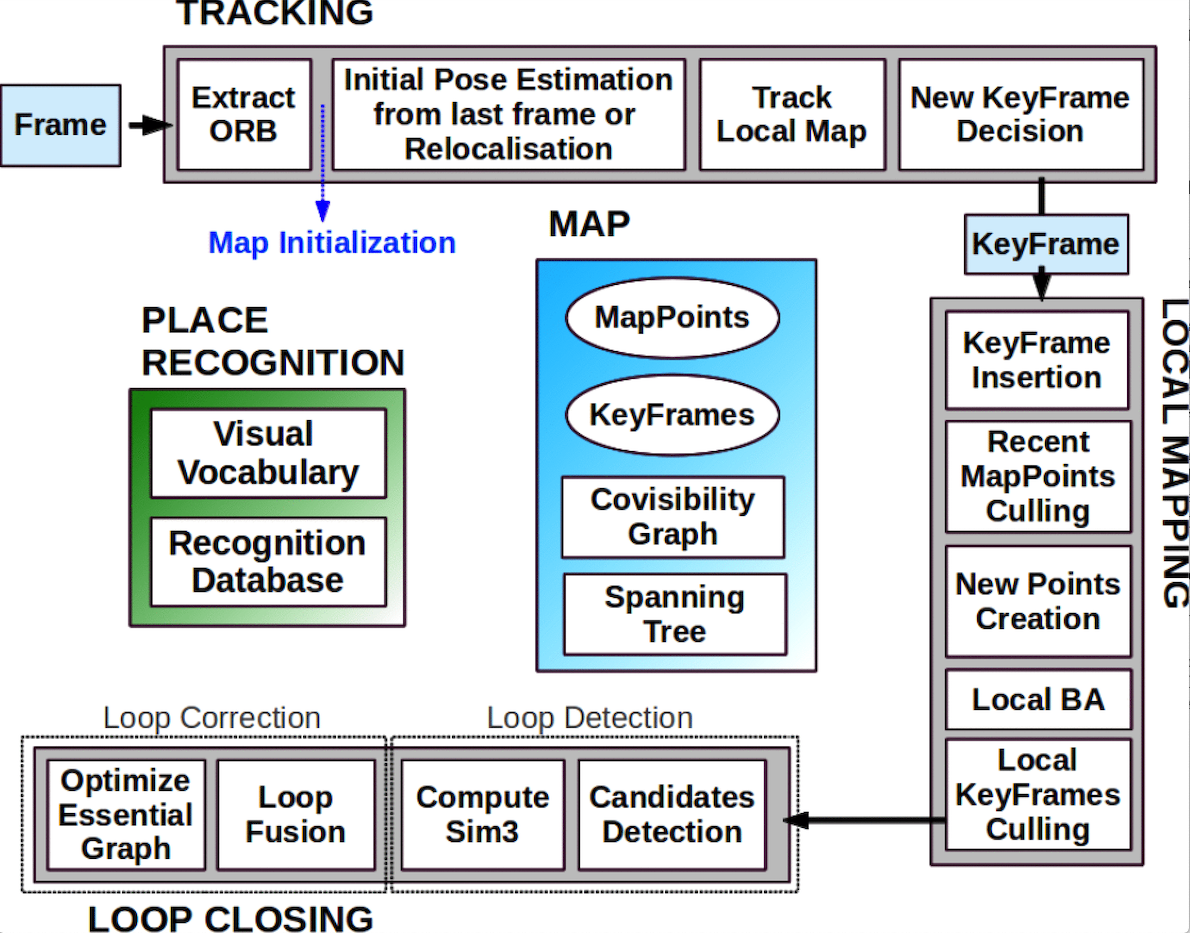
\includegraphics[width=4in]{Chapter2/ORBSLAMOverview.eps}
\caption{ORB-SLAM system overview.}
\label{fig:orbslamoverview} 
\end{figure}

\subsection{CORB-SLAM}
\cite{li2017corb}
\begin{figure}[H]
\centering
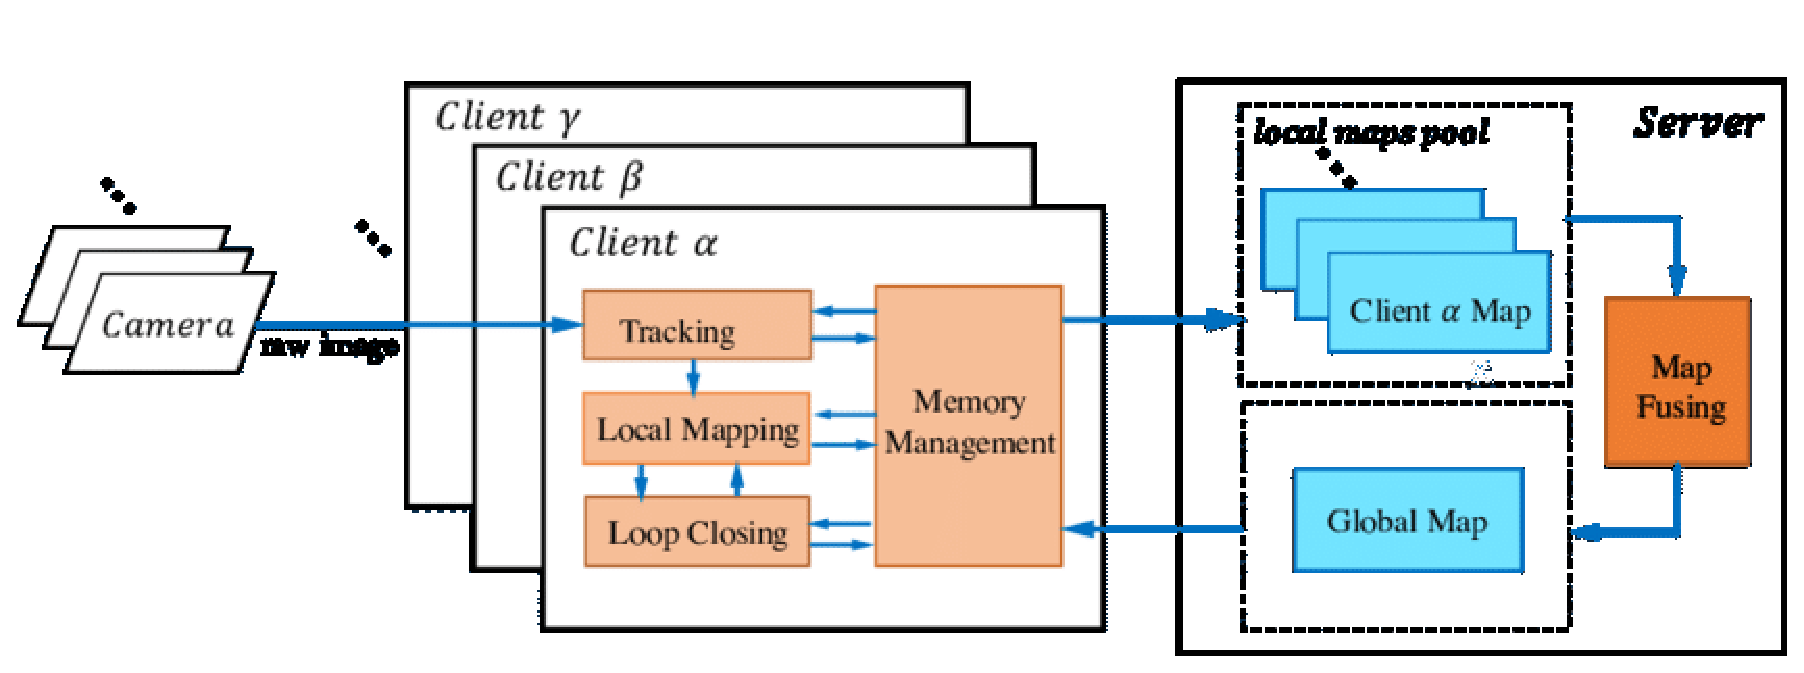
\includegraphics[width=4in]{Chapter2/CORBSLAMOverview.eps}
\caption{The framework of CORB-SLAM system.}
\label{fig:corbslamoverview} 
\end{figure}

\section{Shade Dealing Algorithms}

\subsection{Model-based Approaches}

\subsection{Illumination Variance}
Model-based shade dealing approaches can remove shade more precise, with fewer image details lost, however, obviously their disadvantages limits their application. Model-based approaches requires the type and position of light sources as a prior information to model the illumination patterns, which process has high computational complexity. But vSLAM systems have significant computational cost already, usually deployed on platforms with limited computation capacity, and in most of cases, vSLAM runs in an indoor or outdoor real-world environment with  information of light sources unknown. Therefore,  these two disadvantage determine model-based approaches are not suitable to be combined with vSLAM.

In the case of vSLAM, considering the requirement of low computational complexity and lower image resolution is acceptable, a simpler approach without modeling is preferred. 

Illumination variance approach proposed in \cite{maddern2014illumination}, is a simple method based on only one equation computing illumination variant images.



 \cite{mcmanus2014shady} \cite{arroyo2016openable}
 
 \begin{equation}
 R^{x,E}=
 \end{equation}
 
\begin{equation}
I=\log(R_2)-\alpha\log(R_1)-(1-\alpha)\log(R_3)
\label{eq:iifinal}
\end{equation}

\subsection{Life-Long SLAM}

\begin{figure}[H]
	\centering
	\includegraphics[width=4in]{Chapter2/COISLAMOverview.eps}
	\caption{Block-flow diagram of the combined stereo localisation approach.}
	\label{fig:coislamoverview} 
\end{figure}

%=== END OF CHAPTER TWO ===
\newpage
